\documentclass{article}
\usepackage{CJK}	%中文支持包
%\usepackage{xeCJK}
%\usepackage{ctex}
%\setCJKmainfont{AR PL UMing CN}
\usepackage{amssymb}%数学符号宏包
\usepackage{graphicx}%图形支持包
\usepackage{float}%浮动图片位置
%\usepackage[bookmarksnumbered=true,colorlinks,linkcolor=black,anchorcolor=blue,citecolor=green,linktocpage=false]{hyperref}
\begin{document}
\begin{CJK}{UTF8}{gbsn}
\title{根据国网检测大纲整理的故障指示器功能}
\author{hanhj}
\maketitle
\newpage
\tableofcontents
\newpage
根据国网检测大纲2017故障指示器的功能整理如下:
检测大纲中故障指示器按照工作原理分成两种,一种是传统型,一种是暂态录波型。
\section{传统型功能要求}
\subsection{短路故障检测}
\par
	\textbf{要求:}\\当线路发生短路故障时,故障指示器应能判断出故障类型(瞬时性或永久性故障),并指示。\\
	\textbf{解读:}\\当线路发生短路故障时,断路器将跳开,此时线路将失电,此条要求故指能够检测出此种状况,要求故指在线路发生短路故障时,能够判别出当前故障是瞬时性还是永久性故障,并指示。\\
	瞬时性或永久性故障的判据是当线路失电后,如果在设定时间内恢复供电,为瞬时性故障,否则为永久性故障。\\
	失电判据:电流低于定值,电压低于定值。\\
	\textbf{原理:}\\
	\footnote{$I_x$是任意相电流,$U_x$是场强}
	失电判据:\\
	\[
		\left\{ 
			\begin{array}{ll}
				I_x<dz\\
				U_x<dz 
			\end{array}
		\right.
	\]
	故障性质判据:\\
		当检测到线路失电后,启动计时,时间到,如果此时恢复供电,且没有故障则为瞬时性故障,否则为永久性故障。这里的故障包括相间短路故障和接地故障。
\subsection{自动检测故障}
\par
	\textbf{要求:}\\应自适应负荷电流大小,当检测到线路电流突变,突变电流持续一段时间后,各相电场强度大幅下降,且残余电流不超过5A,应能就地采集故障信息,就地指示故障,且能将将故障信息上传到主站。\\
	\textbf{解读:}\\此条要求实际是要求故指能判断线路短路故障即失电故障。即断路器在线路发生短路故障时,将跳开,此时线路将失电,此时要求故指能够检测这种状况。原理与上面的失电判断原理一致,只是加上时间要求。\\
	\textbf{原理:}
	\footnote{$I_x$是任意相电流,$I_z$是残余电流,$U_x$是场强,$U_{dz}$可以取0.3U,U为故障前的场强。}
	\begin{equation}	
		\left\{ \begin{array}{ll}
				\Delta I_x>I_{dz} & \textrm{启动条件}\\
			    t>T_{dz} & \textrm{突变电流持续的时间}\\
				I_z<5A & \textrm{持续时间后,剩余电流}\\ 
			\Delta U_x>U_{dz}
		\end{array}
		\right .
	\end{equation}
\subsection{接地故障检测和告警}
	\par
	\textbf{要求:}\\当线路发生接地故障时,故指应能够以外施加信号检测法,暂态特征检测法,稳态特征检测法等方式检测接地故障。\\
	\textbf{解读:}	\\稳态特征就是检测$I_0$的大小,外施加信号和暂态特征检测法参见暂态型说明。\\
	\textbf{稳态特征识别原理:}\\
	\begin{equation}
		\left\{
			\begin{array}{ll}
				I_0>I_{dz} & \textrm{零序电流大小}\\
				  t>T_{dz} & \textrm{持续时间}
			\end{array}
			\right.
	\end{equation}
\subsection{故障后复归}
	\par
	\textbf{要求:}\\
	架空型应能在规定时间或线路恢复正常供电后自动复位,也可根据故障性质(永久性或瞬时性)自动选择复归方式。\\
	电缆型应能在手动、规定时间或线路恢复供电自动复归。也可根据故障性质自动选择复归方式。\\
	\textbf{解读:}\\
	当检测到故障后(失电故障或接地故障),此时终端要指示故障,那么何时消除故障,则有几种方式。\\
	1)按照时间消除:即从检测出故障开始计时,等到一定时间后即消除指示。\\	
	2) 线路恢复供电后消除:即一旦检测到恢复供电即消除。\\
	3) 手动消除。\\
	以上几种方式,不能自动切换,即设定什么方式就是什么方式。为了利用所检测到的故障性质,还有一种自动方式,即按照故障性质来消除。可以这样来设定:当是瞬时性故障时,按照时间复归;当是永久性故障时,按照自动恢复供电复归。手动复归方式优先于前两种方式。\\
	瞬时还是永久性故障针对的是短路故障,即失电故障。如果采用恢复供电复位,为了避免误复位(重合闸涌流,或重合后后加速),需要在检测到恢复供电后等一段时间,这个时间不大于5min。\\
	对于接地故障,当检测到故障后,断路器可能不会跳开,因此此时线路仍然供电,但是存在零序电压(即如果是单相接地有两相电压高,一相电压低。)故障,此时不会复位。只有电压电流恢复(电压恢复是指恢复到故障前电压,电流恢复是指大于残余电流),且没有零序电压故障时,认为供电恢复,等一段时间后执行复位。\\
	\textbf{原理:}\\
	略

\subsection{ 低电量告警}
	\par
	\textbf{要求:}\\
	架空型采集单元应能以翻牌锁死方式指示电池低电量。电缆型采集单元、显示面板均以变化色卡颜色指示低电量。\\
	\textbf{解读:}\\
	这个没有什么好说的,就是检测电池电压,加上机械动作。\\
	\textbf{原理:}\\
	略
\subsection{ 防误动}
	\par
	\textbf{要求:}\\
	负荷波动不应误报警;变压器空载合闸涌流不应误报警;线路突合负载涌流不应误报警;人工投切大负荷不应误报警;非故障相重合闸涌流不应误报警。\\
	\textbf{解读:}\\
	这些要求是一些原则性要求,具体到实现,对于相间短路故障,由于检测的是断路器跳闸后的失电情况,因此对于以上情况并不存在(因为都不会引起失电)。对于接地故障,有可能导致零序电流过大,此时可以通过延时来解决。具体来说,当检测到接地故障,可以等待一段时间,再进行检测一次,如果此时零序电压依然存在(或者$\Delta U_x>U_{dz}$),则确认为接地故障,否则认为是误报。\\
	\textbf{原理:}\\
	略
\subsection{ 重合闸识别}
	\par
	\textbf{要求:}\\
	1)应能识别间隔为0.2s的瞬时性故障,并正确动作;\\
	2) 非故障线路安装的故指经受0.2s重合闸间隔停电后,在感受到重合闸涌流后不应误动作。\\
	\textbf{解读:}\\
	第一个要求实际上是对检测时间分辨率的要求,即至少能够分辨到0.2s;第二个要求与上面的防误动要求一致。具体实现方法同上。\\
	\textbf{原理:}\\
	略
\subsection{ 监测和管理}
	\par
	\textbf{要求:}\\
	1)汇集单元至少能够满足3条线路(每条线路3只)采集单元的接入要求。\\
	2) 应具备历史数据存储能力,包括不少于256条的事件顺序记录,30条本地操作记录,10条装置异常记录。\\
	3) 应具备本地及远方维护功能,支持远方程序升级。\\
	\textbf{解读:}\\
	第一条实际上是对硬件cpu运算速度要求,要求能够实时采集至少9个采集单元信息,并进行计算。第二条是对硬件存储容量的要求。第三条是要求具备远程升级功能。\\
	\textbf{原理:}\\
	这个没有什么好说的。
\subsection{ 带电装卸}
	\par
	\textbf{要求:}\\
	架空型应具有带电装卸功能,装卸过程中不应误报警。\\
	\textbf{解读:}\\
	这个要求与防误动情况一样,实现方法同防误动。\\
	\textbf{原理:}\\
	略
\subsection{ 通讯功能}
	\par
	\textbf{要求:}\\
	1)应能通过无线通信方式主动上送告警信息,复归信息以及监测的负荷电流,故障数据等信息至配电主站,故障信息上送至主站时间应小于60s,并支持主站召测全数据功能。\\
	2)具备对时功能,接收主站或其他时间同步装置的对时命令,与系统时钟保持同步。守时精度2s/24h.\\
	3)当后备电池电压降低到阈值时,应将其状态上传至主站,也可根据需要进行本地报警。当外部电源失去时,后备电源应能自动无缝投入,且保证将失电前的完整的故障数据上传至主站。\\
	4)采集单元与汇集单元之间应能以无线、光纤灯方式进行通讯。无线方式宜采用微功率方式。\\
	5)汇集单元应适应无线传输要求,在网络中断后,具有本地存储和调用模式,保存故障信息等关键数据。\\
	6)汇集单元可以通过实时在线或准实时在线方式与配电主站通信,并能以不大于24h的间隔上传负荷曲线数据至主站。\\
	\textbf{解读:}\\
	1)这个实际是对规约以及数据项的要求。具体来说支持101,104规约,支持101平衡方式的主动上送数据或非平衡方式的事件收集方式上送事件;支持104规约中的主动上送数据。支持总召唤。数据项包括遥信数据,包括各种告警信息,复归信息。遥测数据:包括负荷数据,支持主动上送变化负荷遥测数据。\\
	2)这个实际上是要求实现101,104规约中的对时功能。守时精度是对硬件的要求。要采用高精度的时钟芯片,并及时调整终端时钟。\\
	3)这个要求遥信数据项中应包括电池低电量告警。后面的要求是对硬件的要求。\\
	4)这个是对通讯方式的选择,在硬件实现时要注意。\\
	5)这个要求是在网络中断后,应当保存未上送的遥信数据,一旦通讯恢复能够上送这些信息。保存可以是保存在内存中,也可以保存在磁盘中。\\
	6)这个包含两个要求。一个是要求保存负荷曲线数据(96点?),一个是能够至少以24h为间隔,上送该数据。前者包括了对存储容量的要求(至少96点的负荷数据,至少支持9个采集单元),数据保存功能实现。后者是要求规约实现负荷曲线上送功能,即文件传输功能。
\subsection{ 电气性能}
	\par
	\textbf{要求:}\\
	1)短路故障报警启动误差不超过$\pm$10\%\\
	2)最小可识别故障电流持续时间不应大于40ms。\\
	3)电缆型故指电缆温度测量误差不大于3°C。\\
	4)低电量告警电压误差不大于$\pm$2\%\\
	5)负荷电流误差负荷以下要求:
	\begin{itemize}
			\item $0\leq I < 100$时,误差为$\pm$3A.
			\item$100\leq I < 600$时,误差为$\pm$3\%。
	\end{itemize}
	6)上电自动复位时间小于5min。定时复位时间可设定,设定范围小于48h,最小分辨率1min(即最大为2880min),定时复位时间误差不超过$\pm$1\%。\\
	7)接地故障识别率:
	\begin{itemize}
			\item 金属性接地达到100\%
			\item 小电阻接地达到100\%
			\item 弧光接地达到90\%
			\item 高阻接地(800$\Omega$以下)达到90\%
	\end{itemize}
	\textbf{解读:}\\
	1,3,4,5是对精度的要求。2是对故障检测时间的要求,即保护计算频率应小于40ms。通常来说,计算的频率是1个周波即20ms。目前一般做法是采集器采集波形,启动故障检测,汇集器进行故障判断。当线路发生故障时,采集器需要启动故障检测,进行录波,并启动通讯,将故障波形发送给汇集器。汇集器接收到故障信号及故障波形后,进行故障判断,识别出故障后,存储数据,并对上通讯。假设故障持续时间为40ms,采集器识别故障时间需要20ms,则留给通讯,汇集器识别故障的时间只有20ms,对于通讯可靠性,实时性,以及计算效率要求较高。此条的要求可能是断路器跳闸较快,防止跳闸了,还没有检测到故障,导致故障指示漏报。6是对复位时间的要求,包括时间精度(最小分辨率,时间误差),功能(定时复位时间可设,上电自动复位时间小于5min)。\\上电自动复位时间,即当检测到失电$->$来电事件后,为了防止上文所说的误动情况,需要等待一段时间,该时间不应大于5min。7是对可靠性的要求,需要通过实验来验证。\\
	\textbf{原理:}\\
	略
\subsection{ 外观 }
	\par
	\textbf{要求:}\\
	具体要求参见检测大纲,比较明了,这里不赘述。

\subsection{ 绝缘性能}
	\par
	\textbf{要求:}\\
	绝缘电阻:电杆固定安装的汇集单元电源回路与外壳之间的绝缘电阻$\geq 5M\Omega$(使用250V绝缘电阻表,绝缘电压$U_i\leq 60V$)。\\
	绝缘强度:电杆固定安装的汇集单元电源回路与外壳之间的额定绝缘电压$U_i \leq 60V$时,施加500V工频电压无击穿,无闪络。\\
	\textbf{解读}\\
	没什么好说的。\\
	\textbf{原理:}\\
	略。

\subsection{ 低温性能}
	\par
	要求同电气性能。
\subsection{ 高温性能}
	\par
	要求同电气性能
\subsection{ 盐雾实验}
	\par
	\textbf{要求:}\\
	在盐雾实验后,外观应无损坏,功能应正常。\\
	\textbf{解读:}\\
	主要是要求材质合格。
\subsection{ 跌落实验}
	\par
	\textbf{要求:}\\
	跌落实验后,外观应无损坏,功能应正常。\\
	\textbf{解读:}\\
	主要是要求材质合格。
\subsection{ 卡线握力实验}
	\par
	\textbf{要求:}\\
	参见检测大纲。\\
	\textbf{解读}\\
	没什么好说的,参见要求。\\
	\textbf{原理:}\\
	略。

\subsection{ 射频磁场实验}
	\par
	\textbf{要求:}\\
	参见检测大纲。\\
	\textbf{解读}\\
	没什么好说的,参见要求。\\
	\textbf{原理:}\\
	略。

\subsection{ 浪涌实验}
	\par
	\textbf{要求:}\\
	参见检测大纲。\\
	\textbf{解读}\\
	没什么好说的,参见要求。\\
	\textbf{原理:}\\
	略。

\subsection{ 脉冲群实验}
	\par
	\textbf{要求:}\\
	参见检测大纲。\\
	\textbf{解读}\\
	没什么好说的,参见要求。\\
	\textbf{原理:}\\
	略。

\subsection{ 阻尼磁场实验}
	\par
	\textbf{要求:}\\
	参见检测大纲。\\
	\textbf{解读}\\
	没什么好说的,参见要求。\\
	\textbf{原理:}\\
	略。

\subsection{ 过量实验}
	\par
	\textbf{要求:}\\
	1)可承受10KV,20kA的短路电流,2s,外观应无损坏,功能应正常。\\
	2)可承受35KV,31.5kA的短路电流,4s,外观应无损坏,功能应正常。\\
	\textbf{解读:}\\
	这个是对互感器的要求。

\subsection{ 临近干扰实验	}
	\par
	\textbf{要求:}\\
	1)当相邻300m线路发生故障时,本线路不应发出误告警\\
	2)本线路发生故障时,相邻300m的导线不应发出本线路正常告警。\\
	\textbf{解读:}\\
	第一条要求即如果有两条线路1,2,假设线路1发生短路或接地故障,线路2没有故障,此时线路2应当没有短路电流或零序电流,此时线路2应当不会发出告警信号。该项要求其实是对可靠性的要求,即不会因相邻线路(300m)出现故障,而导致出现本线路误报。但是终端检测故障实际上是对本线路的电信号进行监测,并不知道是否有相邻线路存在,如果由于线路1的故障导致线路2的电信号也呈现故障特征,则无法识别。所以本条要求并不是很合理,只是要求终端能够抗干扰信号,对于由于故障线路所产生的例如涌流,脉冲群等干扰信号不至于发生误报警。\\
	第二条要求实际上是对通讯可靠性的要求,因为故障信号的采集来自于采集单元,然后发送到汇集单元,如果发生故障时,线路距离较远(300m),有可能由于故障信号所引发的干扰信号导致通讯出现异常,进而导致不能正确采集信号,而导致不能告警。
\\
所以这两条要求实际上是在终端满足前面常规模拟干扰实验后的再次实际检验。
\subsection{ 着火实验}
	\par
	\textbf{要求:}\\
	采集单元和架空线悬挂的汇集单元外壳应当采用非金属阻燃材料,能够承受5级着火危险。\\
	\textbf{解读:}\\
	本条要求就是对材质的要求。没什么好说的。
\subsection{ 电源及功率消耗实验}
	\par
	\textbf{要求:}\\
	1)线路负荷电流不小于10A时,TA取电5s内应能满足全部功能要求。\\
	2)采集单元非充电电池单独供电时,最小工作电流应不大于40uA。\\
	3)采用太阳能供电的汇集单元电池充满电后额定电压不低于DC12V。采用TA取电的汇集单元电池额定电压不低于DC3.6V。\\
	4)就地型故指采集单元、显示面板静态功耗应小于15uA;远传型故指采集单元功耗应小于40uA,汇集单元整机正常工作功耗应不大于5VA。\\
	\textbf{解读:}\\
	总结一下:\\
	取电方式可以有TA取电,太阳能取电,电池供电。这里没有PT取电,因为不可能在终端上再加装PT。采集器一般采用TA取电,加上小型的后备电池(因为需要翻牌指示)。汇集器一般采用TA取电或太阳能取电,如果用TA取电要在加上后备电池,用太阳能一般配置了后备电池。由于受到体积限制,对于采集器后备电池不可能太大,对于汇集器来说,后备电池可以稍大。\\
	关于功耗的要求包括工作电流,整机功耗,额定电压。总的来说要求是低功耗,因为没有PT供电,对于采集器,如果采用TA取电,负荷电流有可能有,当失电时没有,此时要靠后备电池支持翻牌指示,而停电时间可能很长(48h,巡线时间),所以要求采集器低功耗。对于汇集器而言,如果采用TA取电,基于上面同样的原因,同样需要低功耗。如果汇集器采用太阳能取电,并不能保证天气良好,所以同样需要低功耗。\\
	对采集器和汇集器有不同的功耗要求。\\
	采集器:
	\begin{itemize}
			\item 非充电电池供电时,最小工作电流不大于40uA。即后备电池是一次性的要求功耗更小。
			\item 就地型采集单元,最小工作电流不大于15uA;远传型采集单元工作电流不大于40uA。就地型是否就是就地有翻牌指示,远传型不就地指示?是否就地型功耗要大一些。
	\end{itemize}
	汇集器:
	\begin{itemize}
			\item 采用太阳能取电的额定电压不小于12V,采用TA取电的额定电压不小于3.6V。这条要求对于额定电压也有限制,防止电压过低,不能正常工作。
			\item 整机功耗不大于5VA。
	\end{itemize}
	除此之外,第一条针对TA取电的,实际上假设开始后备电池没电,此时TA送电后,要求充电且能工作的时间不大于5s。\\
	\textbf{原理:}\\
	略
\subsection{ 防护等级:}
	\par
	\textbf{要求:}\\
	采集单元,悬挂安装的汇集单元防护等级不低于IPX7。\\
	电杆固定安装的汇集单元防护等级不低于IPX5。\\
	\textbf{解读:}\\
	IP第一个数字表示对危险的防护,阻止人对危险物体的靠近。这里X表示没有危险。第二个数字表示对进水的防护,7表示短时浸水,5表示喷水。6表示猛烈喷水。\\
	实验的满足条件实验后,不影响正常操作,不产生破坏。水不积聚,不进入带电部分。\\
	\textbf{原理:}\\
	没什么好说的,外壳密封。

\section{暂态录波型功能要求}
\subsection{ 短路和接地故障识别}
	\par
	\textbf{要求:}\\
	1)应自适应负荷电流大小,当检测到电流突变且突变启动值不低于150A,突变电流持续一段时间后,各相电场强度大幅下降,且残余电流不超过5A零飘值,应能就地采集故障信息,以闪光形式就地指示故障,且能将故障信息上传至主站。\\
	2)发生接地故障,当指示器不能判断出接地故障处于安装位置上游和下游时,采集单元应能就地采集故障信息和波形,且能将故障信息和波形上传至主站进行判断,同时汇集单元应能接收主站下发的故障数据信息,采集单元以闪光形式指示故障;\\
	当指示器能够判断出接地故障处于安装位置的上游和下游时,采集单元应能就地采集故障信息和波形,以闪光形式就地指示故障,且能将故障信息和波形上传至主站。\\
	3)接地故障判别适应中性点不接地,经消弧线圈接地,经小电阻接地等配电网中性点接地方式;满足金属性接地、弧光接地、电阻接地等不同接地故障检测要求。\\
	4)当线路发生故障后,采集单元应能正确识别故障类型,并能够根据故障类型选择复位形式。
	\begin{itemize}
			\item 能识别重合闸间隔为不小于0.2s的瞬时性和永久性短路故障,并正确动作。
			\item 线路永久性故障恢复后上电自动延时复位,瞬时性故障后按设定时间或执行主站远程复位。
	\end{itemize}
	\textbf{解读1:}\\
	对于第一条,要求检测短路故障,实际同传统型一样,就是检测线路失电状况,其检测原理同上。只不过这里确定了一个参数就是$\Delta I$的定值不低于150A\\
	\textbf{原理1:}
	\footnote{$I_x$是任意相电流,$I_z$是残余电流,$U_x$是场强。}
	$$	
		\left\{ \begin{array}{ll}
				\Delta I_x>I_{dz} & \textrm{启动条件}\\
			    t>T_{dz} & \textrm{突变电流持续的时间}\\
				I_z<5A & \textrm{持续时间后,剩余电流}\\ 
			\Delta U_x>U_{dz}
		\end{array}
		\right.
	$$
	\textbf{解读2:}\\
	对于第二个要求,这里实际包括以下几个要求:1)要能够判断出接地故障。2)要能够判断出接地故障是在安装处的上游还是下游。3)要显示故障。4)要记录故障波形,即录波功能。5)上传主站故障波形和遥信信息。这就要求终端支持文件传输功能,上传事件功能。6)支持根据主站下发判断信息,显示故障功能(闪光)。这里包括支持命令或参数设置要求(根据规约),以及动作。\\
	3,4,5,6没有什么好说的根据规约和判断结果进行动作。重点是1,2。\\
	\textbf{1)如何判断出接地故障。}\\
	当前供电局接地形式主要包括以下几种:1、直接接地。直接接地一般用于110KV以上场合。2、通过电阻接地。包括小中高电阻接地。3、不接地。4、通过消弧线圈接地。在配电网中2,3,4形式都有可能。还有一种是动态电阻方式,即平时不接地,当检测到绝缘故障时,人为投入小电阻接地,以增大零序电流,利于故障检测的方式。接地故障可能有以下几种形式:1,从接地的阻值来分,可有低阻(包括金属性接地),中阻,高阻接地;2,从接地状态来分可有永久性接地,间歇性接地(包括弧光接地)。\\
	从当前继电保护原理来说接地保护包括以下几种方法:
	\begin{itemize}
			\item 零序电流保护:原理是比较稳态零序电流幅值,适用于中性点接地系统,不接地或小电阻接地系统(能可靠检测出永久性金属性接地,低阻接地状况)。
			\item 零序电流方向保护:原理是比较稳态零序电流方向幅值,非故障线路零序电流方向母线由流向线路,故障线路零序电流方向由线路流向母线,利用此特点可以区分故障线路和非故障线路。对于中性点接地系统,对于双或多电源系统可以保证选择性。对于中性点不接地或小电阻接地系统(能可靠检测出永久性金属性接地,低阻接地状况,且并能判断出故障方向,进而判断出故障线路)。贾总提出的零序相位保护与此类似,不过是在此基础上检测相位,即使是非故障线路与故障线路同方向,但是相位可能不同,从而区分出故障线路和非故障线路。但是对于经消弧线圈接地系统,由于通常采用过补偿方式,补偿后的故障线路零序电流方向与非故障线路方向相同,失去了选择性,而且补偿后的零序电流较小,只有几安,检测比较困难。以上两种方式比较的都是稳态零序电流,当发生间歇性接地,比如弧光接地时,零序电流大小不定,方向也可能不定,可能不能可靠检测到故障。
			\item 绝缘监视: 原理是对于非直接接地系统,由于当发生单相接地故障时,连在同一母线上的线路故障相相电压降低,非故障相相电压升高,利用此特点可以判断出系统出现接地故障,但是不能选出故障线路。
			\item 暂态特征保护\cite{p1}。原理是利用单相接地时的零序电压变化启动检测,原理1:利用暂态电流幅值较稳态电流幅值大几倍到几十倍的特征来检测故障。原理2:利用零序电流$i_0$与$du_0/d_t$(即零序电压导数)之间的线性关系k来判断:对非故障线路或检测点位于故障点下游,k为正;故障线路中检测点位于故障点上游k为负。采用暂态特征保护可以适应中性点不接地以及消弧线圈接地的系统,因为其暂态特征相似。但是对于原理1来说,是假设接地故障是发生在零序电压最大值的时候,如果接地故障发生在零序电压过零点,则暂态电流较小,原理上存在一些漏洞。\\
				以暂态特征实现故障检测的故障指示器,实现时需要解决的几个问题:
				\begin{enumerate}
				\item  取电问题,或者说低功耗问题,原因是没有pt可供电。
				\item  数据同步问题。由于三个采集器采集负荷电流,相电压,交给汇集器计算零序电流,零序电压,所以需要三个采集器采样同步。方法可以是汇集器定时向采集器发送对时命令,采集器收到命令后调整采样中断。但是由于低功耗原因,不能频繁启动通讯,为此需要汇集器在接收到采集器数据后,对数据进行处理偏移,以保证数据同步。
				\item 零序电压采集。由于无法安装pt,所以采集器通过电容来感应相电压,此电压绝对值并不重要,因为在故指中需要的是相电压的变化量。可以通过故障相电压降低或非故障相电压升高来启动故障判断。
				\item 零序电流采集。目前故障指示器往往采用罗氏线圈来采集相电流。罗氏线圈可以将电流转换成微分信号,终端通过积分电路还原信号。积分用的运放可以采用opa2379,其具有精度高,低功耗特点。罗氏线圈是将双绞线缠绕在非磁性材料上,具有抗干扰性好,范围宽,无饱和等优点。
				\item 采样频率。由于需要采集暂态信号,所以采样速率必须高。发生故障时,暂态过程一般持续$5\sim 20ms$,尖峰持续1ms左右。为此可以采用16K的采样频率,1ms可以采集16个点,可以比较好的还原暂态信号,但是所带来的问题是存储容量加大,为此可以在平时用4K的采样频率,故障时采用16K的采样频率。
				\item  通讯。采集器与汇集器之间往往通过微功率无线传输,需要解决通讯可靠性以及传输距离与功耗之间的矛盾问题。
			\end{enumerate}
		\item 其他几种保护方法:国内还曾经出现以下几种保护方法:\cite{p2}
			\begin{itemize}
					\item 首半波法。利用暂态过程中首半波零序电压与零序电流方向一致的方法判断。但是其假设接地故障发生在相电压最大时候,当接地故障发生在零序电压过零点的时候,这个条件不存在。因此存在误报情况。
					\item 五次谐波法。利用暂态过程中5次谐波占比较大特点判断。但是实际效果并不很好。
					\item 信号注入法。原理是在变电站加装信号注入装置,当检测到绝缘故障时,向故障线路故障相注入信号,只有故障线路的故障相能感受到该信号,从而判断出故障线路。但是该方法投资较大,增加系统复杂性。
			\end{itemize}
	\end{itemize}
	\textbf{2)如何判断出故障位于安装处的上游或下游}\\
			假设本机号为0,上游故指号为1,下游故指号为2。当检测出线路故障后,故障指示器可以向相邻的故障指示器发送询问命令,如果相邻的故障指示器均返回故障信号,则说明故障点不位于本地。如果有1号故障指示器返回故障信号,2号故障指示器返回无故障信号,则说明故障点位于本机与2号之间。如果1号返回无故障信号,2号返回故障信号,则说明故障位于本机与1号之间。\\
	\textbf{原理2}\\
	\footnote{$U_x$是相电压,$i_0(k)$是零序电流序列,$u_0(k)$是零序电压序列,$x(k)$是首半波零序电流序列,$y(k)$是首半波零序电压导数序列,N是1个周波采样点数,如果采用16KHz采用频率,则N为320点,n为80点。K是计算的相关系数,计算5次取3次。$U_{dz}$可以取0.3U,U是故障前电压。}
	\par
		$$
			\left\{	
				\begin{array}{ll}
				\Delta U_x>U_{dz} & \textrm{启动条件}\\
				i_0(k)=i_a(k) + i_b(k) + i_c(k) & k=0...N \\
				u_o(k)=u_a(k)+u_b(k)+u_c(k) & k=0...N \\
				x(k)=i_0(k) & k=0...N/4 \\
				y(k+1)=u_0(k+1)-u_0(k) & k=0...N/4 \\
				K(i)=\frac{n\sum{x_i y_i}-\sum x_i\sum y_i}{n\sum x_i^2 - \sum x_i \sum y_i} & i=1...5\\
				\end{array}
			\right.
		$$
		当计算$K>0$时说明无故障,$K<0$时说明有故障。\\
		检测过程流程图参见图1。\\
		\begin{figure}[H]
		\centering
		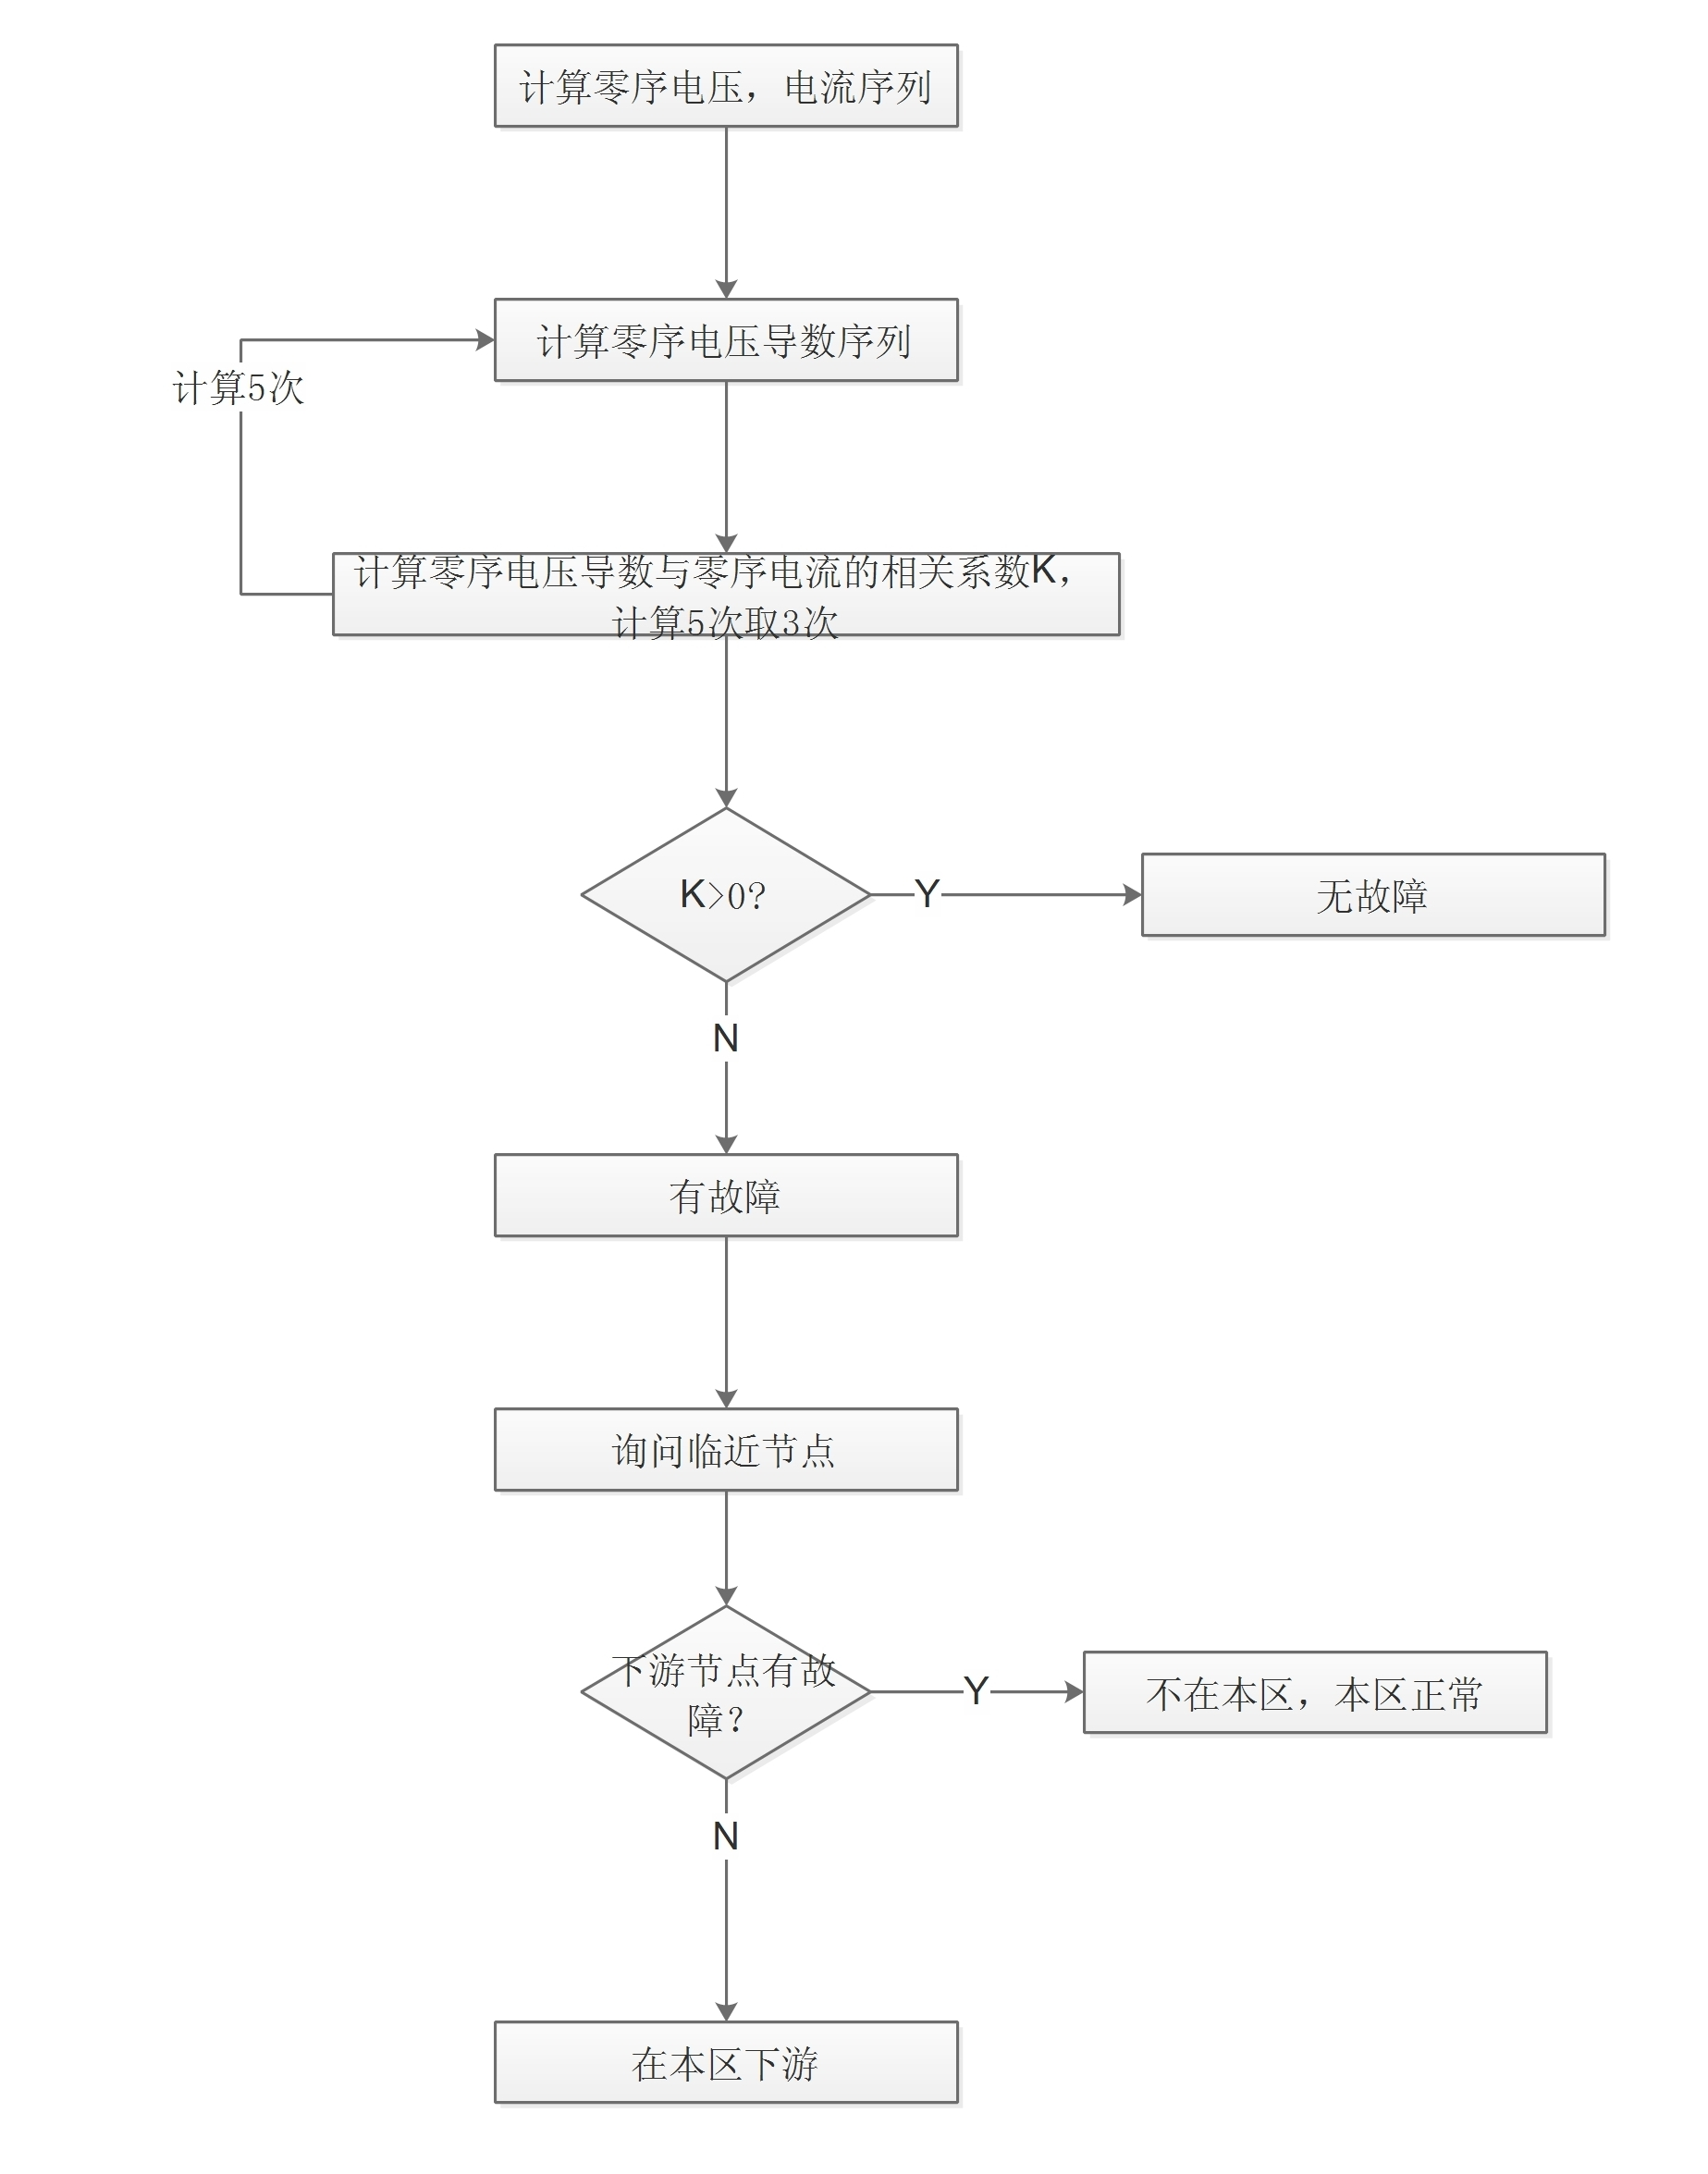
\includegraphics[scale=0.4]{figure1.jpg}
		\caption{检测过程流程图}
		\end{figure}
		\textbf{解读3:}\\
		根据\cite{p1},暂态特征检测法可以适应中性点接地,消弧线圈接地,小电阻接地,并能满足金属性接地,弧光接地,低阻接地的状况。\\
		\textbf{原理3:}\\
		参见原理2的描述。\\
		\textbf{解读4:}\\
		参见传统型的1,4条解读。\\
		\textbf{原理4:}\\
		略
\subsection{ 监测功能}
		\par
		\textbf{要求:}\\
		应能监测线路三相负荷电流、故障电流、相电场强度等运行信息和主供电电源、后备电源等状态信息,并将以上信息上传至主站,同时采集单元具备故障录波功能。\\		\textbf{解读:}\\
		这些都是些常规要求,在满足保护原理基础上对故障信息以及运行信息进行保存,上送。\\
		\textbf{原理:}\\
		略
\subsection{ 故障录波功能}
		\par
		\textbf{要求:}
			\begin{enumerate}
				\item 故障发生时,采集单元应能实现三相同步录波,并上送至汇集单元合成零序电流波形,用于故障的判断。 
				\item 录波范围包括不少于启动前 4 个周波、启动后 8 个周波,每周波不少于80 个采样点,录波数据循环缓存。 
				\item 汇集单元应能将 3 只采集单元上送的故障信息、波形,合成为一个波形文件并标注时间参数上送给主站,时标误差小于 100μs。 
				\item 录波启动条件可包括电流突变、相电场强度突变等,应实现同组触发、阈值可设。 
				\item 录波数据可响应主站发起的召测,上送配电主站的录波数据应符合
				\item Comtrade 1999 标准的文件格式要求,且只采用 CFG 和 DAT 两个文件,并且采用二进制格式。 
		\end{enumerate}
		\textbf{解读:}\\
		按照字面可以很好理解。这里需要注意的是要求b中提到采集点数每周波不少于80点,即采样频率至少为4KHz。其他按照要求来做就是。
\subsection{ 防误报警功能 }
		\par
		\textbf{要求}
		\begin{enumerate}
		\item 负荷波动不应误报警。 
		\item 大负荷投切不应误报警。 
		\item 合闸(含重合闸)涌流不应误报警。 
		\item 采集单元、悬挂安装的汇集单元带电安装拆卸不应误报警。 
		\end{enumerate}
		\textbf{解读:}\\
		这些要求与传统型的要求基本一致,参见传统型第6项的解读。


\subsection{ 数据存储功能 }
		\par
		\textbf{要求:}
		\begin{enumerate}
		\item 汇集单元可循环存储每组采集单元的电流、相电场强度定点数据、64 条故障事件记录和 64 次故障录波数据,且断电可保存,定点数据固定为 1 天 96个点。 
		\item 支持采集单元和汇集单元参数的存储及修改,断电可保存。 
		\item 具备日志记录及远程查询召录功能,日志内容及格式应按照附件 5。 
		\end{enumerate}
		\textbf{解读:}\\
		没什么好说的,按照规约与数据项要求实现。有一点就是需要计算汇集单元的存储器容量。

\subsection{ 远程配置和就地维护功能 }
		\par
		\textbf{要求}
		\begin{enumerate}
		\item 短路、接地故障的判断启动条件。 
		\item 故障就地指示信号的复位时间、复位方式。 
		\item 故障录波数据存储数量和汇集单元的通信参数。 
		\item 采集单元上送数据至汇集单元时间间隔和汇集单元上送数据至主站时间间隔。 
		\item 采集单元故障录波时间、周期和汇集单元历史数据存储时间。 
		\item 汇集单元、采集单元备用电源投入与告警记录。具备自诊断功能,应能检测自身的电池电压,当电池电压低于一定限值时,上送低电压告警信息。 
		\item 汇集单元支持通过无线公网远程升级,采集单元支持接收汇集单元远程程序升级,升级前后应功能兼容。 
		\end{enumerate}
		\textbf{解读:}\\
		数据项的要求,按照要求实现。

\subsection{ 通信试验 }
		\par
		\textbf{要求}
		\begin{enumerate}
		\item 采集单元应支持实时故障、负荷等信息召测,同时并能根据工作电源情况定期或定时上送至汇集单元。 
		\item 采集单元定时发送信息给汇集单元,汇集单元在 10min 内没有收到采集单元信息,即视为通信异常。采集单元与汇集单元通信故障时应能将报警信息上送至配电主站。 
		\item 可通过配电主站对汇集单元和采集单元进行参数设置。 
		\item 汇集单元应支持数据定时上送,最小上送时间间隔为 15min。 
		\item 汇集单元应支持主站及北斗或其他同步时钟装置对时,守时精度≤2s/24h。		
		\end{enumerate}
		\textbf{解读:}\\
		这里提了一条采集器与汇集器之间的通讯故障遥信。\\
		终端要实现历史数据存储,规约中的总召唤,事件收集,文件传输,参数设置,对时功能。以及时钟精度要求。
\subsection{ 电气性能		}
		\par
		\textbf{要求}
			\begin{enumerate}
				\item 短路故障报警启动误差应不大于±10\%。 
				\item 最小可识别短路故障电流持续时间应不大于 40ms。 
				\item 接地故障识别正确率: 
					\begin{enumerate}
						\item 金属性接地应达到 100\%。 
				    	\item 小电阻接地应达到 100\%。 
				    	\item 弧光接地应达到 90\%。 
				    	\item 高阻接地(1kΩ以下)应达到 90\%。 
					\end{enumerate}
				\item 负荷电流误差应符合以下要求:
					\begin{enumerate}
						\item  0≤I<300 时,测量误差为±3A。 
				    	\item 300≤I<600 时,测量误差为±1\%。 
					\end{enumerate}
				\item 上电自动复位时间小于 5min。定时复位时间可设定,设定范围小于48h,最小分辨率为 1min,定时复位时间允许误差不大于±1\%。 
				\item 录波稳态误差应符合以下要求: 
					\begin{enumerate}	
						\item 0≤I<300时,测量误差为±3A。 
						\item 300≤I<600 时,测量误差为±1\%。 
					\end{enumerate}
				\item 故障录波暂态性能中最大峰值瞬时误差应不大于 10\%。 
				\item 故障发生时间和录波启动时间的时间偏差大不于 20ms。 
				\item 每组采集单元三相合成同步误差不大于 100μs。 
		\end{enumerate}
		\textbf{解读:}\\
		1,4,6,7是对测量电压,测量电流精度的要求,注意这里对负荷电流精度的要求与传统型不一样,转折点在300A,传统型在100A,转折点以上传统型要求3\%,这里要求1\%。2要求检测算法不应太长,最多2个周波。3是通过实际检验效果。5,8,9是要求时钟精度。
\subsection{ 外观 }
	\par
	\textbf{要求:}\\
	具体要求参见检测大纲,比较明了,这里不赘述。

\subsection{ 绝缘性能}
	\par
	\textbf{要求:}\\
	绝缘电阻:电杆固定安装的汇集单元电源回路与外壳之间的绝缘电阻$\geq 5M\Omega$(使用250V绝缘电阻表,绝缘电压$U_i\leq 60V$)。\\
	绝缘强度:电杆固定安装的汇集单元电源回路与外壳之间的额定绝缘电压$U_i \leq 60V$时,施加500V工频电压无击穿,无闪络。\\
	\textbf{解读}\\
	没什么好说的。\\
	\textbf{原理:}\\
	略。

\subsection{ 低温性能}
	\par
	要求同电气性能。
\subsection{ 高温性能}
	\par
	要求同电气性能
\subsection{ 盐雾实验}
	\par
	\textbf{要求:}\\
	在盐雾实验后,外观应无损坏,功能应正常。\\
	\textbf{解读:}\\
	主要是要求材质合格。
\subsection{ 跌落实验}
	\par
	\textbf{要求:}\\
	跌落实验后,外观应无损坏,功能应正常。\\
	\textbf{解读:}\\
	主要是要求材质合格。
\subsection{ 卡线握力实验}
	\par
	\textbf{要求:}\\
	参见检测大纲。\\
	\textbf{解读}\\
	没什么好说的,参见要求。\\
	\textbf{原理:}\\
	略。

\subsection{ 射频磁场实验}
	\par
	\textbf{要求:}\\
	参见检测大纲。\\
	\textbf{解读}\\
	没什么好说的,参见要求。\\
	\textbf{原理:}\\
	略。

\subsection{ 浪涌实验}
	\par
	\textbf{要求:}\\
	参见检测大纲。\\
	\textbf{解读}\\
	没什么好说的,参见要求。\\
	\textbf{原理:}\\
	略。

\subsection{ 脉冲群实验}
	\par
	\textbf{要求:}\\
	参见检测大纲。\\
	\textbf{解读}\\
	没什么好说的,参见要求。\\
	\textbf{原理:}\\
	略。

\subsection{ 阻尼磁场实验}
	\par
	\textbf{要求:}\\
	参见检测大纲。\\
	\textbf{解读}\\
	没什么好说的,参见要求。\\
	\textbf{原理:}\\
	略。

\subsection{ 过量实验}
	\par
	\textbf{要求:}\\
	1)可承受10KV,20kA的短路电流,2s,外观应无损坏,功能应正常。\\
	2)可承受35KV,31.5kA的短路电流,4s,外观应无损坏,功能应正常。\\
	\textbf{解读:}\\
	这个是对互感器的要求。

\subsection{ 临近干扰实验	}
	\par
	\textbf{要求:}\\
	1)当相邻300m线路发生故障时,本线路不应发出误告警\\
	2)本线路发生故障时,相邻300m的导线不应发出本线路正常告警。\\
	\textbf{解读:}\\
	第一条要求即如果有两条线路1,2,假设线路1发生短路或接地故障,线路2没有故障,此时线路2应当没有短路电流或零序电流,此时线路2应当不会发出告警信号。该项要求其实是对可靠性的要求,即不会因相邻线路(300m)出现故障,而导致出现本线路误报。但是终端检测故障实际上是对本线路的电信号进行监测,并不知道是否有相邻线路存在,如果由于线路1的故障导致线路2的电信号也呈现故障特征,则无法识别。所以本条要求并不是很合理,只是要求终端能够抗干扰信号,对于由于故障线路所产生的例如涌流,脉冲群等干扰信号不至于发生误报警。\\
	第二条要求实际上是对通讯可靠性的要求,因为故障信号的采集来自于采集单元,然后发送到汇集单元,如果发生故障时,线路距离较远(300m),有可能由于故障信号所引发的干扰信号导致通讯出现异常,进而导致不能正确采集信号,而导致不能告警。
\\
所以这两条要求实际上是在终端满足前面常规模拟干扰实验后的再次实际检验。
\subsection{ 着火实验}
	\par
	\textbf{要求:}\\
	采集单元和架空线悬挂的汇集单元外壳应当采用非金属阻燃材料,能够承受5级着火危险。\\
	\textbf{解读:}\\
	本条要求就是对材质的要求。没什么好说的。
\subsection{ 电源及功率消耗实验}
	\par
	\textbf{要求:}\\
	1)线路负荷电流不小于5A时,TA取电5s内应能满足全部功能要求。线路负荷电流低于5A,且超级电容失去供电能力时,应至少判断短路故障,定期采集负荷电流,并上传至汇集单元。\\
	2)采集单元非充电电池单独供电时,额定电压应不小于DC3.6V。在电池单独供电时,最小工作电流应不大于80uA。\\
	3)采用太阳能供电的汇集单元电池充满电后额定电压不低于DC12V。采用TA取电的汇集单元电池额定电压不低于DC3.6V。\\
	4)汇集单元整机正常工作功耗(在线,不通信)应不大于0.2VA。\\
	\textbf{解读:}\\
	\underline{与传统型相比,暂态型汇集单元的功耗更低,0.2VA(传统型是5VA)。}\\
	采集器:
	\begin{itemize}
			\item 非充电电池供电时,应该是纽扣电池,估计是不好测,所以要求供电电压。采用充电电池的,要求最小工作电流不大于80uA,比传统型一次性电池的40uA大。
	\end{itemize}
	汇集器:
	\begin{itemize}
			\item 采用太阳能取电的额定电压不小于12V,采用TA取电的额定电压不小于3.6V。这条要求对于额定电压也有限制,防止电压过低,不能正常工作。
			\item 整机功耗不大于0.2VA。
	\end{itemize}
	除此之外,第一条针对TA取电的,实际上假设开始后备电池没电,此时TA送电后,要求充电且能工作的时间不大于5s。而且当负荷电流过小,且后备电池失去作用时,允许接地故障判断功能丧失。实际上可能此时采集单元进入低功耗模式,检测接地故障需要实时检测电压,电流,而短路故障只要检测电压降低信号,所以可以减小一些功耗。\\
	\textbf{原理:}\\
	略
\subsection{ 防护等级:}
	\par
	\textbf{要求:}\\
	采集单元,悬挂安装的汇集单元防护等级不低于IPX7。\\
	电杆固定安装的汇集单元防护等级不低于IPX5。\\
	\textbf{解读:}\\
	IP第一个数字表示对危险的防护,阻止人对危险物体的靠近。这里X表示没有危险。第二个数字表示对进水的防护,7表示短时浸水,5表示喷水。6表示猛烈喷水。\\
	实验的满足条件是水不影响正常操作,产生破坏。水不积聚,不进入带电部分。\\
	\textbf{原理:}\\
	没什么好说的,外壳密封。
	
\begin{thebibliography}{99}
\bibitem{p1}肖小兵,徐长宝,黄亮亮等. 适用于小电流接地系统的暂态特征型故障指示器技术研究(J). 电子器件. 2018,41(2):333-338
\bibitem{p2}吕常智,陈勇. 适用于架空线路的接地型故障指示器检测方法研究(J). 电子测试. 2016,11
\end{thebibliography}
\end{CJK}
\end{document}

